\graphicspath{{lit_study/fig/}}

{
\tikzset{external/figure name/.add={lit_study/}{}}


\chapter{Literature study}
\label{chap:lit_study}

\section{Payload transportation with multirotors}

    \paragraph
    The transportation of payloads with \glspl{UAV} has significantly grown in popularity over recent years.
    % Examples of specific applications of \gls{UAV} transportation include package deliveries \cite{}, pesticide application in agriculture \cite{}, and 
    Multirotor \glspl{UAV} are specifically useful for many transportation applications due to their agility, and their \gls{VTOL} and hover capabilities.
    The types of payloads attached to multirotors can usually be categorised as either sensors (e.g. cameras and meteorological sensors), or freight (e.g. mail parcels or fire extinguishing material) \cite{Vergouw2016}.
    Furthermore, the payload attachment is mainly categorised as either a rigid connection, or a cable-suspended connection \cite{Vergouw2016}.
    In rare cases, a robotic actuator is attached to the multirotor to manipulate the payload \cite{Gonzalez-deSantos2020} \cite{Suthar2021}.
    The payload attachment and the physical properties of the payload influence the flight dynamics of a multirotor and needs to be considered for control system design.   
    In many applications, some aspects of the payload configuration are unknown prior to flight and the control architecture needs to account for these unknowns.

    % figure of rigid and suspended payload

    \subsection{Rigidly attached payloads}

        \paragraph
        Payloads are often rigidly attached to a multirotor for transportation.
        This configuration is especially popular for commercial package deliveries \cite{San2018}.
        There is minimal relative movement between the multirotor and the rigidly connected payload, hence, the payload only affects the \gls{CoM}, the moment of inertia, and the aerodynamics of the vehicle.
        Often, the weight and size of the payload is unknown prior to flight.
        
        \paragraph
        Different control approaches have been proposed to deal with the altered flight dynamics for this applications, 
        including \gls{ARC} \cite{Min2011} and \gls{MRAC} \cite{Emran2015}.
        These control architectures mostly involve a parameter estimation algorithm to estimate the inertial parameters,
        and an adaptive control law which is based on the estimated parameters and a dynamical model of the system.

        % \paragraph
        % \author{Mellinger2011a} \cite{Mellinger2011a} proposed an adaptive controller for a multirotor with a rigidly connected payload.
        % Least-squares estimation techniques were applied to estimate the inertial parameters of the payload.
        % A adaptive control law was then applied which uses the estimated parameters in the control law.
        % Experimental results showed acceptable trajectory tracking performance with the adaptive controller.

        \paragraph
        An advantage of rigidly connected payloads is that the flight dynamics are not altered significantly.
        The payload does not add a degree of freedom to the system and only the inertial parameters need to be account for.
        However, this configuration limits the shape and size of a potential payload, since
        the payload needs to be compatible with the vehicle gripper.
        The multirotor also needs to land or approach the payload very closely to attach to the load, which may be impractical in many applications.

    \subsection{Cable-suspended payloads}

        \paragraph
        Figure~\ref{fig:real_suspended_payload_example} shows an example of a practical application of a suspended payload used during search and rescue missions.
        The shape and mass of the payload has an effect on the flight dynamics, but the payload is often unknown prior to flight.
        The control system should be able to account for these uncertainties and fly well despite the altered flight dynamics.

        \begin{figure}[htb]
            \centering
            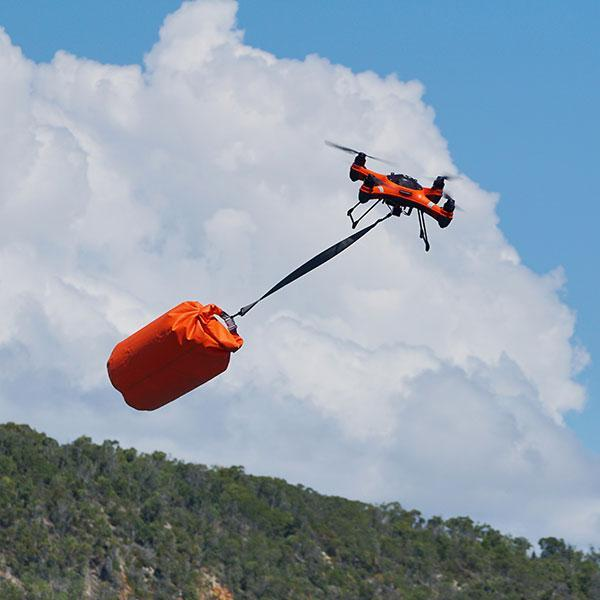
\includegraphics[width=0.45\linewidth]{real_suspended_payload_example.jpg}            
            \caption{A practical suspended payload used for search and rescue missions \cite{CompareCommander2020}}
            \label{fig:real_suspended_payload_example}
        \end{figure}

        \paragraph
        Various suspended payload configurations have been considered in literture.
        Elastic
        Taut
        multiple drones.
        However, in many situations a single multirotor is sufficient to transport the load
        
        \paragraph
        Cable-suspended attachments are very useful in situations where the multirotor cannot land, since the payload can be attach during hover.
        This configuration also has the advantage that a load can have an arbitrary shape or size as long as it has an attachment point for a cable.
        However, the suspended payload increases the degrees of underactuation of the system, which makes the control problem challenging \cite{Kotaru2018}.

        % Active vs passive attachments
        % https://hybrid-robotics.berkeley.edu/publications/ACC2017_QuadLoad_ElasticCable.pdf
        % In terms of mechanical design, several methods have been
        % proposed to attach a payload to a UAV, involving both active
        % and passive attachments. Examples of active attachments
        % include using actuated grippers to grip and pickup payloads
        % [13], [10], and actuated manipulator arms to enable aerial
        % manipulation [10]. These active mechanisms provide more
        % degrees-of-freedom (DOFs) to the UAV, and help in active
        % aerial manipulation. However, these advantages come at
        % the cost of loss of agility of the small UAVs due to the
        % added inertia to the system. Moreover, actuated gripper arms
        % introduce dynamic coupling between the manipulator and
        % quadrotor which needs to be accurately captured in the
        % mathematical model and compensated by the controller.
        % Passive type of attachments have also been developed,
        % wherein the payload is attached to the UAVs through a mechanical cable or tether [2], [15], [17], [6], [18]. By attaching
        % the payload through tethers, the payload could be connected
        % to a single or multiple UAVs without directly modifying the
        % UAV’s inertia. However, this becomes more challenging for
        % control due to the additional degree-of-underactuation. Early
        % work looked at the transportation of a single point-mass load
        % 1P. Kotaru, G. Wu are with Department of Mechanical Engineering,
        % Carnegie Mellon University, 5000 Forbes Avenue, Pittsburgh PA, 15213,
        % email: {vkotaru,gwu}@andrew.cmu.edu.
        % K. Sreenath is with the Depts. of Mechanical Engineering, The Robotics
        % Institute, and Electrical and Computer Engineering, Carnegie Mellon University, Pittsburgh, PA 15213, email: koushils@cmu.edu.
        % This work is supported in part by the Google Faculty Research Award
        % and in part by NSF grants CMMI-1538869, IIS-1464337, IIS-1526515.
        % Fig. 1: Quadrotor with load through a suspended cable, with
        % the cable modeled as a spring-damper. The configuration
        % space of the system is given as R
        % 3 × SO(3) × S
        % 2 × R,
        % with 9 degrees-of-freedom and 4 actuators, resulting in 5
        % degrees-of-underactuation.
        % with single and multiple helicopters [2], with the objective
        % being to actively cancel any swing in the cable. Furthermore,
        % dynamic programming (DP) based methods were employed
        % to plan dynamically-feasible trajectories that minimized the
        % load swing along with an adaptive controller in [15].



\section{Control of a multirotor with a suspended payload}

    \subsection{Input shapers}

    \subsection{Active-damping controllers}

    
    % ?? Lit study: include different types of \gls{MPC}, e.g. DMC, MAC
    % ?? different types of models \cite{}, 
    % ?? See \cite{Garcia1989} for good example of different implementations with different models
 

\section{System identification of a multirotor with an unknown suspended payload}

   
% \section{System Design}
% Blok diagram
% komponente

}


